\noindent There are two urns, one red and one blue, each containing 4 balls as displayed below. All balls are labeled with a letter 'I', the meaning of which will be explained on the next page. One of the two urns will be randomly selected in the beginning. You do not know which urn will be selected. It will remain the same throughout this study. 

\vspace{1cm}
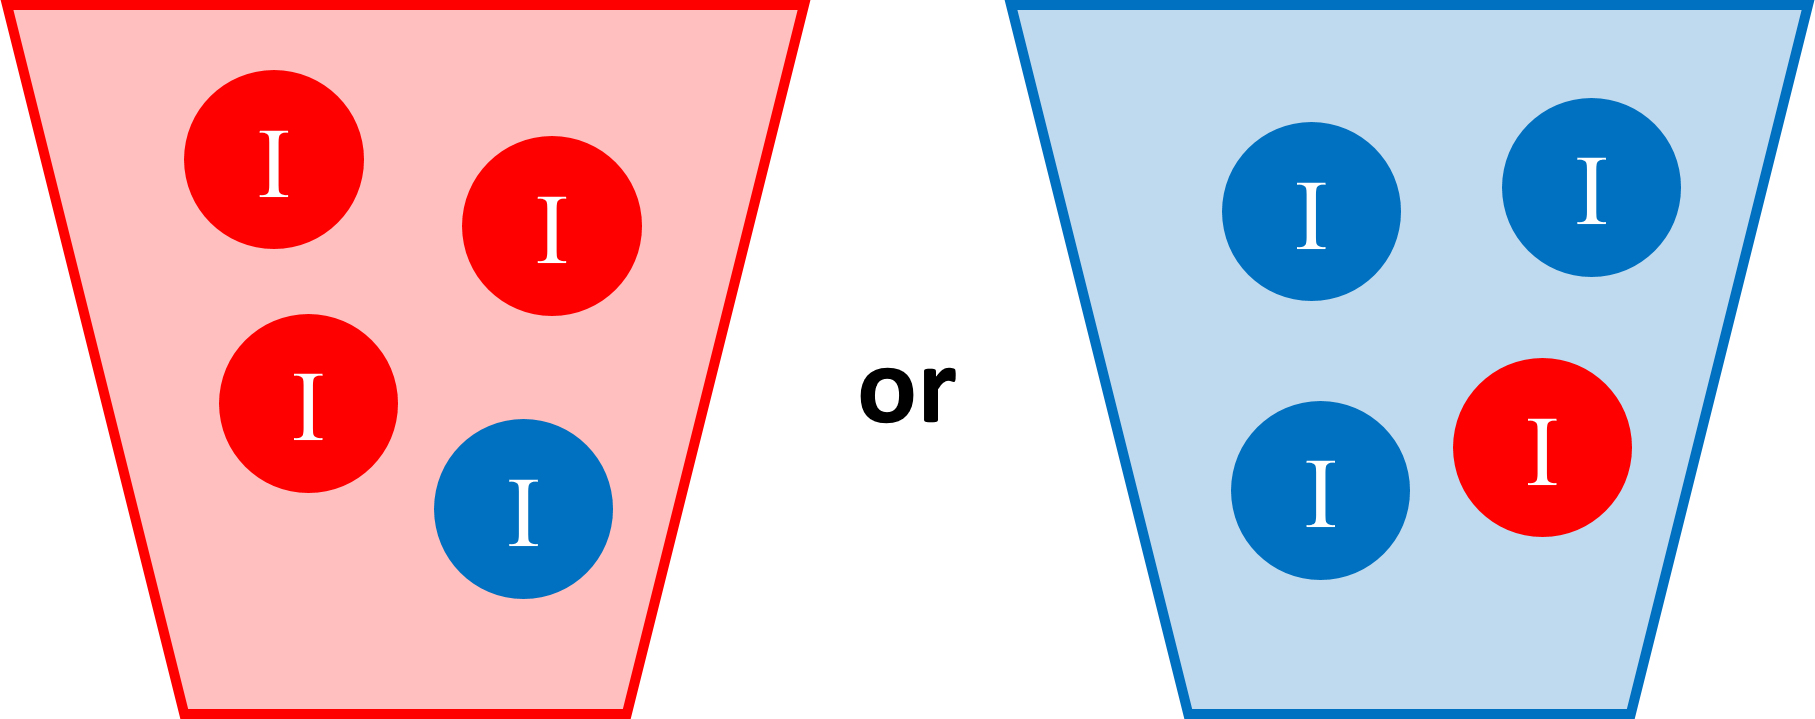
\includegraphics[width=8cm]{instructions/red_or_blue_urn.png}
\vspace{1cm}

\noindent Your \textbf{task will be to guess which urn you think was selected.} To do so you will receive hints about the selected urn. This will be described on the next page. 

-------------------------------------- [Page break] --------------------------------------

\noindent The selected urn contains 4 balls, 3 of the same color and 1 of the opposite color, as shown on the previous page. All balls from the selected urn are put into a black box. They are labeled with the letter 'I', which stands for 'informative'. If you knew the colour of all 4 balls, you would be able to identify the selected urn. For the moment you do not know the color of the selected urn and therefore the 4 informative balls are displayed in grey (although they have a color, either red or blue). 

\noindent The black box also contains 6 other balls that do not come from the urn. These 6 balls are labeled with the letter 'U', which stands for 'uninformative'. Knowing the color of the uninformative balls does not help to identify the selected urn. \textbf{The black box and the 10 balls inside it remain the same throughout the entire study. }

\vspace{1cm}
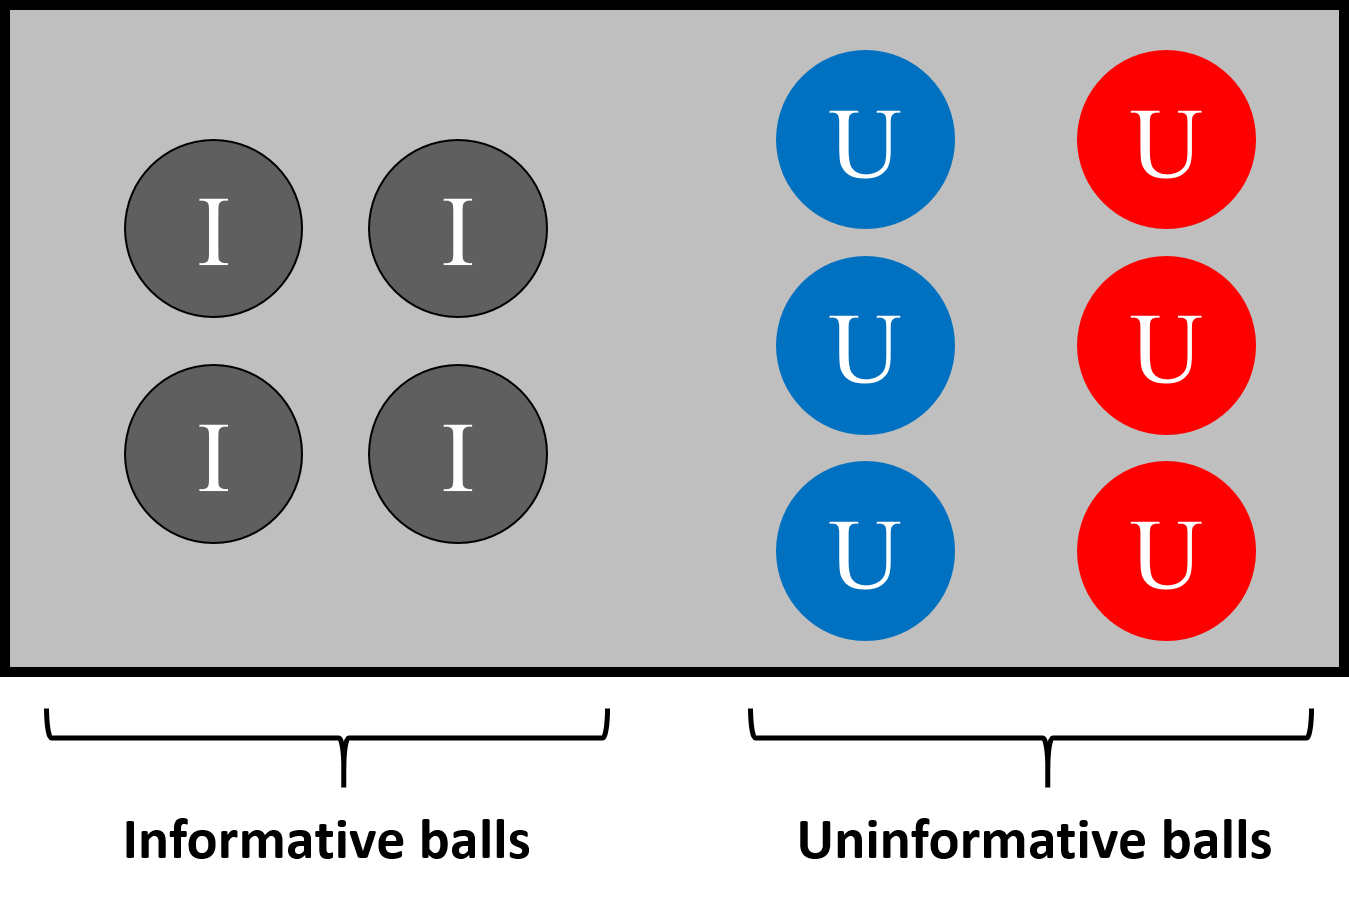
\includegraphics[width=8cm]{instructions/black_box.png}
\vspace{1cm}

This study has 12 rounds in total. In each round you get one of two possible hints: 
\begin{itemize}
    \item \textbf{A ball is drawn} from the black box. You are told the color of the ball. The ball is put back into the box together with the other 9 balls. You do not know if the balls is informative or uninformative. \textit{Example:} A red ball is drawn from the box. 
\includegraphics[width=0.5cm]{instructions/red_ball_q.png}
    \item No new ball is drawn, but you receive \textbf{information about the ball you saw previously}. You will be told if the ball you saw before was one of the 4 informative balls or one of the 6 uninformative balls. \textit{Example:} Previously you saw a red ball. The ball that was drawn last round was one of the 6 uninformative balls. 
\includegraphics[width=0.5cm]{instructions/red_ball_u.png} 
\end{itemize}

\noindent In every round you will be asked to make a guess about the urn that has been selected in the beginning. At the end of the study you will be told the color of this urn. You will receive a bonus which depends on the accuracy of your answer to one of the 12 guesses (you do not know which one). The procedure for calculating your bonus is described in detail below. You may skip these details. The important thing is that the procedure guarantees that you should expect to maximize your bonus by reporting what you truly think the chances are in each question. 

-------------------------------------- [Button: 'Details about the bonus'] --------------------------------------

\noindent\textbf{We apply the following procedure: 
}

\noindent First, we randomly pick one of the questions. For this question, we calculate the error you made. This is how many percentage points your report was away from 100\% (if the RED URN was selected) or from 0\% (if the BLUE URN was selected). Then, we plug in the error into the following formula: 

$$3-3 \cdot \text{error}^2$$

 \noindent This will be your bonus (in Euros). 

\noindent\textbf{EXAMPLE:} Suppose that you report 60\% chance that the RED URN was selected in Step 1. Then, your bonus is calculated as follows: 
\begin{itemize}
    \item If the urn was RED:
    \begin{itemize}
        \item your error is $(100\%-60\%) = 40\%$
        \item your bonus is $3-3\cdot (40\%)^2 = 2.52 \text{Euros}$
    \end{itemize}
    \item If the urn was BLUE:
    \begin{itemize}
        \item your error is $(60\%-0\%) = 60\%$
        \item your bonus is $3-3\cdot (60\%)^2 = 1.92 \text{Euros}$
    \end{itemize}
\end{itemize}

\noindent As we have already mentioned, you should expect to maximize your earnings by reporting what you actually think are the chances of a RED URN. 

\noindent \textbf{Example:} If you actually think that the chances are 60\% that the RED URN was selected, then:
\begin{itemize}
    \item By reporting 60\%, you will make on average 2.28 Euros.
    \item By reporting 10\%, you will make on average 1.53 Euros.
    \item By reporting 100\%, you will make on average 1.80 Euros.
\end{itemize}

\noindent As you see you maximize your earning by reporting exactly 60\%. The further away you report from what you actually think, the less money you should expect to make.


